%! Author = alanmiranda
%! Date = 05/11/2022

% Preamble
\documentclass[a4paper, 11pt]{article}

% Packages
\usepackage[portuguese]{babel}
\usepackage{amsmath}
\usepackage{graphicx}
\usepackage{setspace}
\usepackage[a4paper, left=2.5cm, right=2.5cm, top=2.5cm, bottom=2.5cm]{geometry}
\usepackage{indentfirst}
\usepackage{listings}
\usepackage{natbib} % Bibliografia
% Document
\singlespacing
\begin{document}
\thispagestyle{empty}
    \begin{center}
        \parbox{3cm}{
\includegraphics[scale=1]{pictures/logo_ufpa}}\\
        \vspace{1cm}
        \Large \uppercase{Universidade Federal do Pará}\\
        \Large \uppercase{Instituto de Tecnologia - ITEC}\\
        \vspace{3cm}
        \Large \uppercase{Faculdade de Engenharia Mecânica - FEM}\\
        \Large \uppercase{Laboratório de Química Analítica Quantitativa - LQAQ}\\
        \vspace{3cm}
        \Large \textbf{\uppercase {Relatório de Prática 7: Utilização de Indicadores Ácidos e Bases}} \\
        \Large \textbf{\uppercase {PROF. DR. Carlos Antônio Neves}} \\
        \vspace{3cm}
        \Large \uppercase {Alan Henrique Pereira Miranda - 202102140072}\\
        \Large \uppercase {Gabriel Cruz de Oliveira - 202102140055}\\
        \Large \uppercase {Paloma Gama da Silva - 202102140029}\\
        \Large \uppercase {Silvio Farias Leal - 202102140035}\\
        \vspace{1cm}
        \Large {Belém-PA \\ 2022}

    \end{center}

\newpage
\section{Introdução}\label{sec:intro}
    \indent A manipulação de ácidos e bases são parte do cotidiano de um químico, e é importante que o mesmo saiba como identificar a presença de um ácido ou base em uma solução, para que possa tomar as medidas de segurança necessárias.\  A utilização de indicadores ácidos e bases é uma forma de identificar a presença de um ácido ou base em uma solução, sem a necessidade de realizar uma titulação.\  Os indicadores ácidos e bases são substâncias que mudam de cor quando expostas a uma solução ácida ou básica, respectivamente.\  A cor de um indicador ácido ou base é chamada de cor de transição, e é a cor que o indicador apresenta quando exposto a uma solução ácida ou básica.\  A cor de transição de um indicador ácido ou base é determinada por sua estrutura química, e é uma característica que não pode ser alterada pelo pH da solução.
    \indent O objetivo deste relatório é identificar a presença de ácidos e bases em soluções, utilizando indicadores ácidos e bases, e determinar a cor de transição de cada indicador utilizado, seguindo as orientações do material de apoio do professor.

\section{Objetivos}\label{sec:objetivos}
    \begin{itemize}
        \item Identificar a presença de ácidos e bases em soluções, utilizando indicadores ácidos e bases.
        \item Determinar a cor de transição de cada indicador utilizado.
    \end{itemize}
    \subsection{Objetivos específicos}\label{sec:objetivos_especificos}
    \indent Verificar o comportamento de cada indicador ácido e base, quando exposto a soluções ácidas e básicas.


\section{Materiais e Métodos}\label{sec:mat}
    \subsection{Materiais}\label{sec:mat_materiais}
    \indent Os materiais utilizados para a realização desta prática foram:
        \begin{table}[h]
        \label{tab:materiais}
        \centering
        \begin{tabular}{|c|c|}
            \hline
            \textbf{Material} & \textbf{Quantidade} \\
            \hline
            Solução de NaOH 0,1 mol/L & 10 mL \\
            \hline
            Solução de HCl 0,1 mol/L & 10 mL \\
            \hline
            Solução de CH$_3$COOH 0,1 mol/L & 10 mL \\
            \hline
            Solução de NH$_4$OH 0,1 mol/L & 10 mL \\
            \hline
            Indicador ácido: Fenolftaleína & 0,15 mL \\
            \hline
            Indicador universal: Azul de bromotimol & 0,15 mL \\
            \hline
            Indicador universal: Alaranjado de metila & 0,15 mL \\
            \hline
            Indicador universal: Papeis de tornassol azul e vermelho & 3 pedaços/amostra \\
            \hline
            Água Sanitária & 10 mL \\
            \hline
            Detergente & 10 mL \\
            \hline
            Suco de limão & 10 mL \\
            \hline
            Suco de Uva & 10 mL \\
            \hline
        \end{tabular}
            \caption{Materiais utilizados neste relatório}
    \end{table}\\
\newpage
    \indent E a seguinte bancada de trabalho:\\
    \begin{figure}[h]
        \centering
        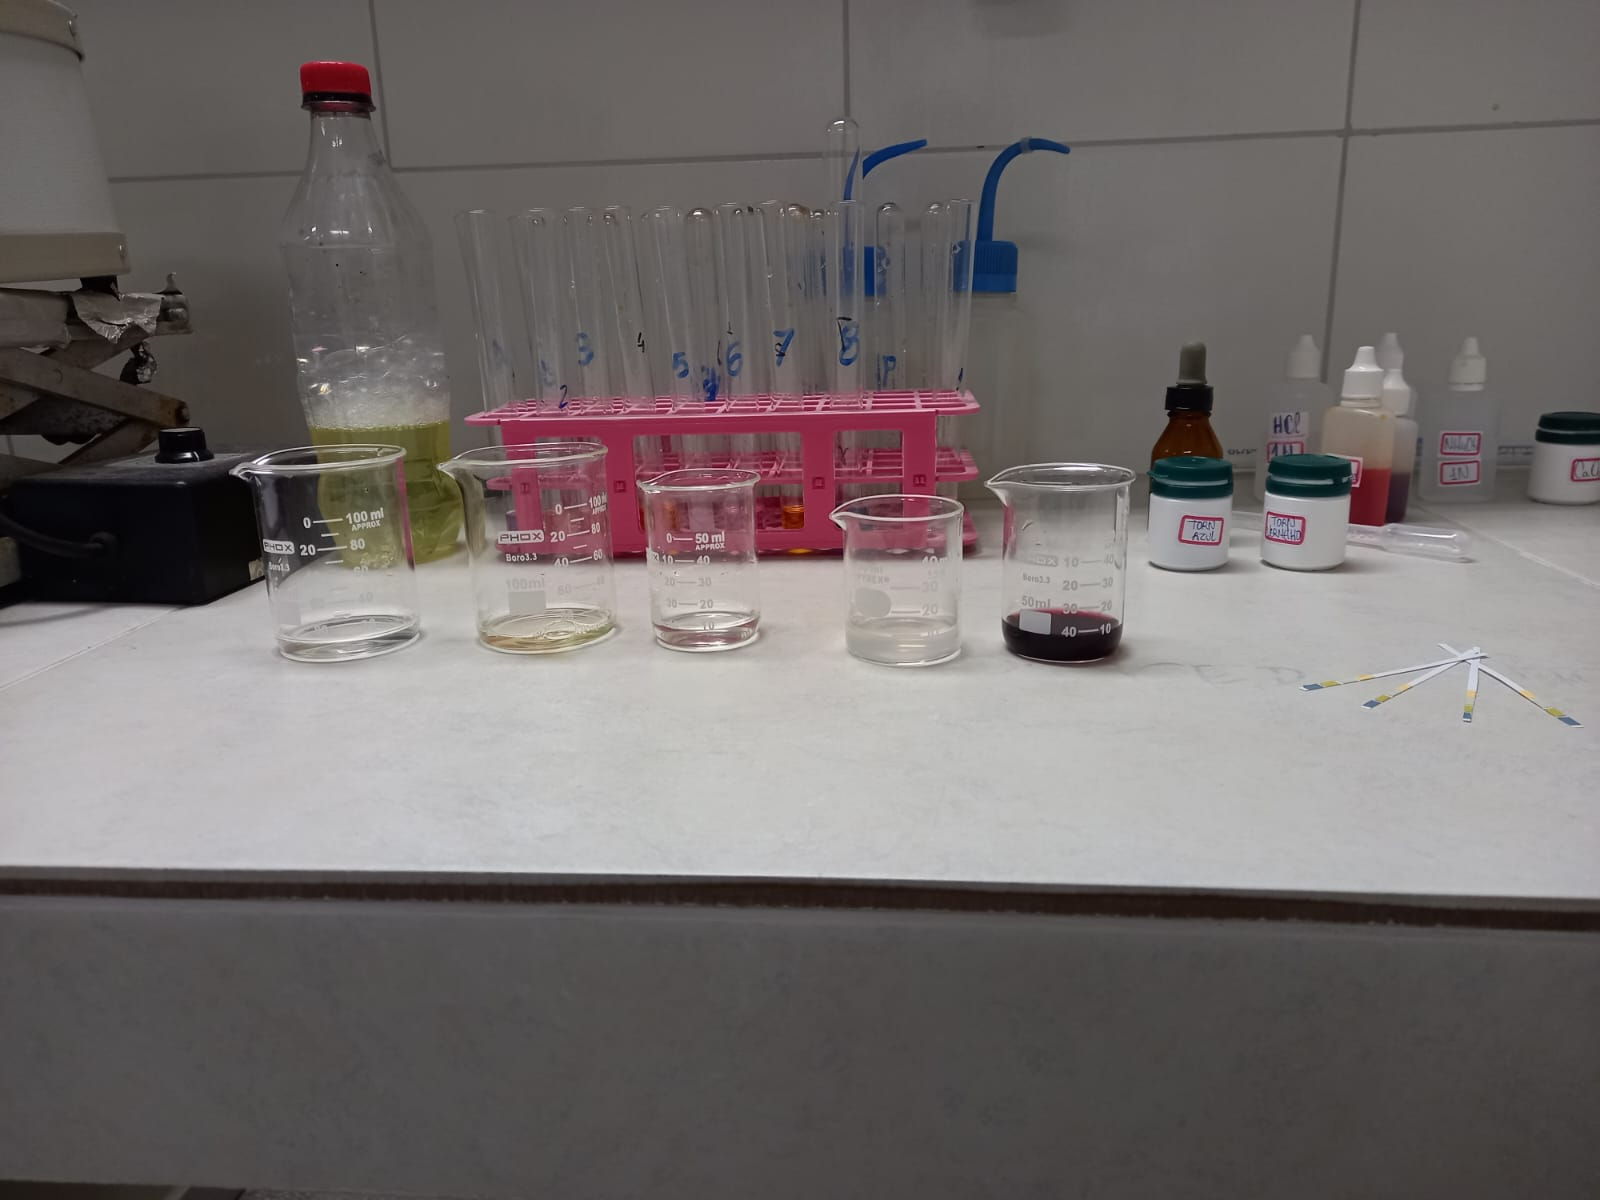
\includegraphics[scale=0.25]{pictures/bancada.jpeg}
        \caption{Bancada de trabalho utilizada para a realização desta prática}\label{fig:figure}
    \end{figure}


\bibliographystyle{unsrt}
\bibliography{bibliografia}
\end{document}